\section{包含, 交与并}\label{sec:inclusions-intersections-unions}

在本节中, 我们讨论 $\mathcal{V}$ 和 $\mathcal{I}$ 算子与集合论概念之间的关系, 先考察它们关于包含关系的性质.

\begin{Proposition}{$\mathcal{V}$ 和 $\mathcal{I}$ 反转包含关系}\leavevmode\label{prop:operators-reverse-inclusions}
  设 $S,T\subseteq K[x_{1},\ldots,x_{n}]$ 和 $X,Y\subseteq\mathbb{A}^{n}$ 为子集.
  \begin{enumerate}[label=\arabic*.,ref=\arabic*]
    \item\label{item:vanishing-set-reverses-inclusion} 若 $S\subseteq T$, 则 $\mathcal{V}(S)\supseteq\mathcal{V}(T)$.
    \item\label{item:vanishing-ideal-reverses-inclusion} 若 $X\subseteq Y$, 则 $\mathcal{I}(X)\supseteq\mathcal{I}(Y)$.
  \end{enumerate}
  此外, 若 $X$ 和 $Y$ 都是仿射簇, 则
  \[
    X\subseteq Y \quad\text{当且仅当}\quad \mathcal{I}(X)\supseteq\mathcal{I}(Y).
  \]
\end{Proposition}

用文字来说, 第一项是说, 较大的多项式集合的公共解比较小的多项式集合的公共解少; 第二项是说, 在 $\mathbb{A}^{n}$ 的较大点集上处处为零的多项式少于在较小点集上处处为零的多项式. 在尝试正式证明之前, 读者不妨花一点时间, 从直观上理解这两个陈述.

\begin{Proof}\unskip\textbf{ of Proposition~\ref{prop:operators-reverse-inclusions}}\quad
  第~\ref{item:vanishing-set-reverses-inclusion}~项和第~\ref{item:vanishing-ideal-reverses-inclusion}~项分别留给 Exercises~\ref{ex:vanishing-sets-reverse-inclusion} 和 \ref{ex:vanishing-ideals-reverse-inclusion}; 这两道习题还说明两个陈述各自的逆命题都可能不成立. 对最后的充要条件, \textquotedbl{}仅当\textquotedbl{}方向就是第~\ref{item:vanishing-ideal-reverses-inclusion}~项的陈述, 因此只需证明\textquotedbl{}当\textquotedbl{}的方向. 于是, 假设 $\mathcal{I}(X)\supseteq\mathcal{I}(Y)$. 由第~\ref{item:vanishing-set-reverses-inclusion}~项得到 $\mathcal{V}(\mathcal{I}(X))\subseteq\mathcal{V}(\mathcal{I}(Y))$. 利用 $X$ 和 $Y$ 都是仿射簇的假设并应用 Proposition~\ref{prop:compose-vanishing-operators}, 可知 $\mathcal{V}(\mathcal{I}(X))=X$ 且 $\mathcal{V}(\mathcal{I}(Y))=Y$, 从而 $X\subseteq Y$.
\end{Proof}

\begin{Example}{双曲面上的一条直线}\leavevmode\label{ex:line-on-a-hyperboloid}
  \BookPairedFigure
    {考虑理想
     \[
       I=\langle x^{2}+y^{2}-z^{2}-1\rangle
       \quad\text{和}\quad J=\langle x-z,y-1\rangle.
     \]
     此时, $\mathcal{V}(I)$ 是\hyperref[fig:line-on-hyperboloid]{右图}所画的 $\mathbb{R}$ 上的单叶双曲面, 簇 $\mathcal{V}(J)$ 是双曲面上那条直线, 其点集形如 $\{(a,1,a)\mid a\in K\}$. 包含关系 $\mathcal{V}(I)\supseteq\mathcal{V}(J)$ 来自理想的包含关系 $I\subseteq J$. 注意到 $I$ 的生成元在 $J$ 中, 即可验证这一点:}
    {\phantomsection\label{fig:line-on-hyperboloid}%
      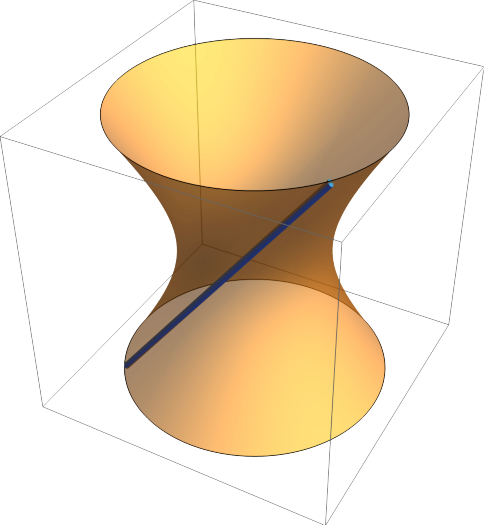
\includegraphics[width=\linewidth]{figures/line-on-hyperboloid.png}}
  \[
    x^{2}+y^{2}-z^{2}-1=(x+z)(x-z)+(y+1)(y-1)\in J.
  \]
\end{Example}

讨论了包含之后, 现在来看交与并. 一族仿射簇的交或并还是仿射簇吗? 如果是, 而且我们恰好知道原来那一族簇的一组定义方程, 能否求出交与并的定义方程? 我们从一个熟悉的例子出发, 探讨这些问题.

\begin{Example}{坐标轴的交与并}\leavevmode\label{ex:coordinate-axes-intersection-and-union}
  考虑仿射簇 $\mathcal{V}(x)\subseteq\mathbb{A}^{2}$ 和 $\mathcal{V}(y)\subseteq\mathbb{A}^{2}$, 它们分别是 $y$ 轴和 $x$ 轴. 两条坐标轴相交于原点. 我们在 Example~\ref{ex:singleton-vanishing-sets} 中看到, 原点由集合 $\{x,y\}$ 同时为零来定义. 因此,
  \begin{equation}\label{eq:coordinate-axes-intersection}
    \mathcal{V}(x)\cap\mathcal{V}(y)=\mathcal{V}(x,y).
  \end{equation}
  另一方面, 它们的并是 Example~\ref{ex:vanishing-set-coordinate-axes} 中的仿射簇, 由多项式 $xy$ 为零来定义. 因此,
  \begin{equation}\label{eq:coordinate-axes-union}
    \mathcal{V}(x)\cup\mathcal{V}(y)=\mathcal{V}(xy).
  \end{equation}
\end{Example}

如果从理想的角度解释等式 \eqref{eq:coordinate-axes-intersection} 和 \eqref{eq:coordinate-axes-union}, 那么等式 \eqref{eq:coordinate-axes-union} 中的理想 $\langle xy\rangle$ 是理想 $\langle x\rangle$ 与 $\langle y\rangle$ 的交. 等式 \eqref{eq:coordinate-axes-intersection} 中的理想 $\langle x,y\rangle$ 并不正好是 $\langle x\rangle$ 与 $\langle y\rangle$ 的并, 因为它们的并不是理想, 而是由这个并集生成的理想 (Exercise~\ref{ex:coordinate-ideals-intersection-and-generated-union}). Example~\ref{ex:coordinate-axes-intersection-and-union} 就这样说明了下面的一般结果.

\begin{Proposition}{零点集的交与并}\leavevmode\label{prop:intersection-and-union-of-vanishing-sets}
  对任意理想 $I,J\subseteq K[x_{1},\ldots,x_{n}]$,
  \[
    \begin{aligned}
      \mathcal{V}(I)\cap\mathcal{V}(J)&=\mathcal{V}(I\cup J),\\
      \mathcal{V}(I)\cup\mathcal{V}(J)&=\mathcal{V}(I\cap J).
    \end{aligned}
  \]
\end{Proposition}

\begin{Proof}
  我们证明第二个等式, 第一个留给 Exercise~\ref{ex:intersection-of-vanishing-sets}.

  ($\subseteq$): 由于 $I\cap J\subseteq I$, Proposition~\ref{prop:operators-reverse-inclusions} 蕴含 $\mathcal{V}(I)\subseteq\mathcal{V}(I\cap J)$. 同理, 有 $\mathcal{V}(J)\subseteq\mathcal{V}(I\cap J)$. 合起来可得
  \[
    \mathcal{V}(I)\cup\mathcal{V}(J)\subseteq\mathcal{V}(I\cap J).
  \]

  ($\supseteq$): 设 $a=(a_{1},\ldots,a_{n})\notin\mathcal{V}(I)\cup\mathcal{V}(J)$. 因为 $a\notin\mathcal{V}(I)$, 所以存在 $f\in I$ 使 $f(a)\ne0$. 类似地, 存在 $g\in J$ 使 $g(a)\ne0$. 因为理想吸收乘法, 乘积 $fg$ 既在 $I$ 中又在 $J$ 中, 所以 $fg\in I\cap J$. 由于
  \[
    (fg)(a)=f(a)g(a)\ne0,
  \]
  可得 $a\notin\mathcal{V}(I\cap J)$, 证明完毕.
\end{Proof}

由于每个仿射簇 $X$ 都是某个理想的零点集, 即理想 $\mathcal{I}(X)$ 的零点集, Proposition~\ref{prop:intersection-and-union-of-vanishing-sets} 蕴含任意两个仿射簇的交与并本身都是仿射簇. 不过, Proposition~\ref{prop:intersection-and-union-of-vanishing-sets} 中的两个等式各有一个不便之处. 在第一个等式中, 问题在于理想的并 $I\cup J$ 一般不是理想 (Exercise~\ref{ex:when-union-of-ideals-is-ideal}). 在第二个等式中, 虽然 $I\cap J$ 是理想, 但在实际运算中可能并不方便. 例如, 即使知道 $I$ 和 $J$ 的生成元, 也不能直接看出怎样求 $I\cap J$ 的生成元.

用下面两种理想的代数运算来重新表述 Proposition~\ref{prop:intersection-and-union-of-vanishing-sets}, 就能解决这两个问题.

\begin{Definition}{理想的和与积}\leavevmode\label{def:sum-and-product-of-ideals}
  设 $I$ 和 $J$ 为环 $R$ 中的理想. $I$ 与 $J$ 的\textbf{和}是理想
  \[
    I+J=\{r+s\mid r\in I,s\in J\},
  \]
  而 $I$ 与 $J$ 的\textbf{积}是理想
  \[
    I\cdot J=\left\{\sum_{i=1}^{m}r_{i}s_{i}\ \middle|\,
      m\in\mathbb{N},r_{i}\in I,s_{i}\in J\right\}.
  \]
\end{Definition}

两个理想的和的定义正如人们所预期的: 把两个理想的元素两两相加所得的集合, 恰好是一个理想. 然而, 积的定义需要额外一步: 由于两两相乘所得的集合对加法不封闭, 要得到一个理想, 就必须把两两乘积的所有有限和都包括进来. 验证两个理想的和与积确实都是理想, 留给 Exercise~\ref{ex:ideal-sum-and-product-properties}; 这道习题还给出了其他一些有用的性质.

处理理想的和与积时, 一个重要之处是: 如果已知 $I$ 和 $J$ 的生成元, 比如 $I=\langle a_{1},\ldots,a_{k}\rangle$ 和 $J=\langle b_{1},\ldots,b_{\ell}\rangle$, 就能直接写出和理想及积理想的生成元 (Exercise~\ref{ex:ideal-sum-and-product-properties}):
\[
  \begin{aligned}
    I+J&=\langle a_{1},\ldots,a_{k},b_{1},\ldots,b_{\ell}\rangle,\\
    I\cdot J&=\langle a_{i}b_{j}\mid i=1,\ldots,k\text{ 且 }j=1,\ldots,\ell\rangle.
  \end{aligned}
\]
例如, 在环 $K[x,y]$ 中, 有
\[
  \begin{aligned}
    \langle x\rangle+\langle y\rangle&=\langle x,y\rangle,\\
    \langle x\rangle\cdot\langle y\rangle&=\langle xy\rangle.
  \end{aligned}
\]
利用和与积, 可以把 Proposition~\ref{prop:intersection-and-union-of-vanishing-sets} 改述如下.

\begin{Proposition}{再论交与并}\leavevmode\label{prop:vanishing-sets-of-ideal-sum-and-product}
  对任意理想 $I,J\subseteq K[x_{1},\ldots,x_{n}]$,
  \[
    \begin{aligned}
      \mathcal{V}(I)\cap\mathcal{V}(J)&=\mathcal{V}(I+J),\\
      \mathcal{V}(I)\cup\mathcal{V}(J)&=\mathcal{V}(I\cdot J).
    \end{aligned}
  \]
\end{Proposition}

\begin{Proof}
  对第一个等式, 只需留意 $I+J$ 是由 $I\cup J$ 生成的理想 (Exercise~\ref{ex:ideal-sum-and-product-properties}), 则 Proposition~\ref{prop:vanishing-sets-of-ideal-sum-and-product} 的第一个等式可由 Proposition~\ref{prop:intersection-and-union-of-vanishing-sets} 的第一个等式得到.

  为证第二个等式, 注意 $I\cdot J$ 包含在 $I$ 和 $J$ 两者之中 (Exercise~\ref{ex:ideal-sum-and-product-properties}). 因此, $\mathcal{V}(I)\cup\mathcal{V}(J)\subseteq\mathcal{V}(I\cdot J)$ 的证明可以原样照搬 Proposition~\ref{prop:intersection-and-union-of-vanishing-sets} 的证明. 类似地, 由于当 $f\in I$ 且 $g\in J$ 时总有 $fg\in I\cdot J$, $\mathcal{V}(I)\cup\mathcal{V}(J)\supseteq\mathcal{V}(I\cdot J)$ 的证明也可原样照用.
\end{Proof}

\begin{Example}{借助理想求交与并}\leavevmode\label{ex:intersection-and-union-via-ideals}
  考虑 $\mathbb{A}^{2}$ 中的仿射簇 $\mathcal{V}(x,y)$ 和 $\mathcal{V}(x-y)$, 它们是原点与过原点的一条直线. 本例用代数方法计算它们的交与并, 验证预期的结果.

  应用 Proposition~\ref{prop:vanishing-sets-of-ideal-sum-and-product} 以及理想的和的生成元描述, 有
  \[
    \mathcal{V}(x,y)\cap\mathcal{V}(x-y)
      =\mathcal{V}(\langle x,y\rangle+\langle x-y\rangle)=\mathcal{V}(x,y,x-y).
  \]
  注意 $\langle x,y,x-y\rangle=\langle x,y\rangle$, 因为 $x-y$ 已在 $x$ 和 $y$ 生成的理想中. 所以上式可写成
  \[
    \mathcal{V}(x,y)\cap\mathcal{V}(x-y)=\mathcal{V}(x,y),
  \]
  它表达了这两个仿射簇的交为原点这一几何事实.

  至于它们的并, Proposition~\ref{prop:vanishing-sets-of-ideal-sum-and-product} 蕴含
  \[
    \mathcal{V}(x,y)\cup\mathcal{V}(x-y)
      =\mathcal{V}(\langle x,y\rangle\cdot\langle x-y\rangle)
      =\mathcal{V}(x(x-y),y(x-y)).
  \]
  元素 $(a,b)\in\mathcal{V}(x(x-y),y(x-y))$ 必须满足方程
  \[
    a(a-b)=0 \qquad\text{和}\qquad b(a-b)=0.
  \]
  第一个方程蕴含 $a=0$ 或 $a=b$. 若 $a=0$, 则第二个方程蕴含 $b^{2}=0$, 所以 $b=0$. 若 $a=b$, 则第二个方程自动满足. 由此可验证
  \[
    \mathcal{V}(x(x-y),y(x-y))=\{(a,b)\in\mathbb{A}^{2}\mid a=b\}.
  \]
  换句话说, 我们用代数方法验证了, 正如预期, 原点与直线 $y=x$ 的并就是这条直线.
\end{Example}

到目前为止, 我们只考虑了两个仿射簇的并与交. 不过细心的读者或许已经发现, 上述一切都可以推广到有限多个仿射簇 $\mathcal{V}(I_{1}),\ldots,\mathcal{V}(I_{k})$ 的并与交. 实际上, 交还可以进一步推广, 允许可数无穷多个仿射簇 $\mathcal{V}(I_{1}),\mathcal{V}(I_{2}),\mathcal{V}(I_{3}),\ldots$, 甚至不可数多个仿射簇.

在记号上, 为了讨论任意一族理想, 我们考虑集合 $\{I_{\alpha}\}_{\alpha\in A}$, 其中 $A$ 是任意集合 (称为指标集), 且对每个 $\alpha\in A$, $I_{\alpha}\subseteq K[x_{1},\ldots,x_{n}]$ 是一个理想. 例如, 如果 $A=\{1,2,3\}$, 这就是一族理想 $\{I_{1},I_{2},I_{3}\}$. 如果 $A=\mathbb{N}$, 这就是可数无穷多个理想 $\{I_{0},I_{1},I_{2},\ldots\}$. 甚至可以取 $A=\mathbb{R}$, 这意味着这一族不仅含理想 $I_{0},I_{1},I_{2},\ldots$, 还含理想 $I_{-1},I_{1/2},I_{\sqrt{2}},I_{\pi}$ 等等.

有了这个记号, 一般结果如下.

\begin{Proposition}{一般的交与并}\leavevmode\label{prop:arbitrary-intersections-and-finite-unions}
  对任意一族理想 $\{I_{\alpha}\}_{\alpha\in A}$, 其中 $I_{\alpha}\subseteq K[x_{1},\ldots,x_{n}]$, 有
  \[
    \bigcap_{\alpha\in A}\mathcal{V}(I_{\alpha})
      =\mathcal{V}\left(\bigcup_{\alpha\in A}I_{\alpha}\right).
  \]
  对任意有限族理想 $\{I_{1},\ldots,I_{k}\}$, 其中 $I_{i}\subseteq K[x_{1},\ldots,x_{n}]$, 有
  \[
    \bigcup_{i=1}^{k}\mathcal{V}(I_{i})
      =\mathcal{V}\left(\bigcap_{i=1}^{k}I_{i}\right).
  \]
\end{Proposition}

\begin{Proof}
  \BookPairedNote
    {证明仿照 Proposition~\ref{prop:intersection-and-union-of-vanishing-sets} 的证明. 第二个等式要求有限性, 是因为 Proposition~\ref{prop:intersection-and-union-of-vanishing-sets} 证明中出现的乘积 $fg$, 在这里要换成从每个 $I_{i}$ 中各取一个 $f_{i}$ 所成的乘积, 而无穷多个多项式的乘积并不是多项式.}
    {Proposition~\ref{prop:arbitrary-intersections-and-finite-unions} 也可以用理想的和与积来表述, 但定义理想的无穷和时需要略加小心.}
\end{Proof}

仿射簇的并要成为仿射簇, 有限性是不可少的. 例如, $\mathbb{Z}\subseteq\mathbb{C}=\mathbb{A}^{1}_{\mathbb{C}}$ 是其中各点的无限并, 每个点都是仿射簇. 但我们知道 $\mathbb{Z}\subseteq\mathbb{A}^{1}_{\mathbb{C}}$ 不是仿射簇, 因为它既不是有限集, 也不是整个 $\mathbb{A}^{1}_{\mathbb{C}}$.

Proposition~\ref{prop:arbitrary-intersections-and-finite-unions} 蕴含仿射簇的任意交与有限并都是仿射簇. 熟悉拓扑学的读者也许会认出这些条件: 连同 $\varnothing$ 和 $\mathbb{A}^{n}$ 都是仿射簇这一事实, 它们构成一个拓扑的闭集的定义条件, 因而闭集的补集构成开集. $\mathbb{A}^{n}$ 上的这一拓扑称为 \textbf{Zariski 拓扑}, 得名于 Oscar Zariski (1899--1986). 他受过经典意大利学派方法的训练, 将这种方法奠定在更严格的代数基础之上, 为现代代数几何作出了奠基性贡献.

虽然本书并不假定读者熟悉拓扑学, 但 Zariski 开集与 Zariski 闭集的术语遍见于代数几何, 所以我们在此给出定义, 以供后文参考.

\begin{Definition}{$\mathbb{A}^{n}$ 上的 Zariski 拓扑}\leavevmode\label{def:zariski-topology}
  若子集 $X\subseteq\mathbb{A}^{n}$ 是仿射簇, 则称 $X$ 是 \textbf{Zariski 闭的}.

  若子集 $U\subseteq\mathbb{A}^{n}$ 的补集 $\mathbb{A}^{n}\setminus U$ 是仿射簇, 则称 $U$ 是 \textbf{Zariski 开的}.
\end{Definition}

\BookPairedNote
  {修饰语\textquotedbl{}Zariski\textquotedbl{}将这个拓扑与 $\mathbb{A}^{n}_{K}$ 上其他自然的拓扑区分开来, 例如 $K=\mathbb{R}$ 或 $\mathbb{C}$ 时的欧氏拓扑.}
  {有拓扑学背景且对此感兴趣的读者, 可参看 Exercise~\ref{ex:compare-zariski-and-euclidean-topologies}, 探索 Zariski 拓扑的一些基本性质及其与欧氏拓扑的比较.}

\BookExerciseHeading
\begin{BookExercises}
  \item\label{ex:vanishing-sets-reverse-inclusion} 设 $S,T\subseteq K[x_{1},\ldots,x_{n}]$ 为子集.
    \begin{enumerate}[label=(\alph*),ref=(\alph*)]
      \item\label{item:vanishing-sets-inclusion-proof} 证明 $S\subseteq T$ 蕴含 $\mathcal{V}(S)\supseteq\mathcal{V}(T)$.
      \item 举例证明 \ref{item:vanishing-sets-inclusion-proof} 的逆命题可能不成立.
    \end{enumerate}
  \item\label{ex:vanishing-ideals-reverse-inclusion} 设 $X,Y\subseteq\mathbb{A}^{n}$ 为子集.
    \begin{enumerate}[label=(\alph*),ref=(\alph*)]
      \item\label{item:vanishing-ideals-inclusion-proof} 证明 $X\subseteq Y$ 蕴含 $\mathcal{I}(X)\supseteq\mathcal{I}(Y)$.
      \item 举例证明 \ref{item:vanishing-ideals-inclusion-proof} 的逆命题可能不成立.
    \end{enumerate}
  \item\label{ex:coordinate-ideals-intersection-and-generated-union} 本题涉及理想 $\langle x\rangle\subseteq K[x,y]$ 与 $\langle y\rangle\subseteq K[x,y]$.
    \begin{enumerate}[label=(\alph*)]
      \item 证明 $\langle x\rangle\cap\langle y\rangle=\langle xy\rangle$.
      \item 证明 $\langle x\rangle\cup\langle y\rangle=\langle x,y\rangle$.
    \end{enumerate}
  \item\label{ex:intersection-of-vanishing-sets} 证明对任意理想 $I,J\subseteq K[x_{1},\ldots,x_{n}]$, 都有
    \[
      \mathcal{V}(I)\cap\mathcal{V}(J)=\mathcal{V}(I\cup J),
    \]
    以补全 Proposition~\ref{prop:intersection-and-union-of-vanishing-sets} 的证明.
  \item\label{ex:when-union-of-ideals-is-ideal} 证明环中两个理想的并是理想, 当且仅当其中一个理想包含在另一个中.
  \item\label{ex:pairwise-products-need-not-be-ideal} 设 $I,J$ 是环 $R$ 的理想. 举例证明 $\{ab\mid a\in I,b\in J\}$ 不一定是 $R$ 的理想.
  \item\label{ex:ideal-sum-and-product-properties} 设 $I$ 和 $J$ 为环 $R$ 中的理想.
    \begin{enumerate}[label=(\alph*)]
      \item 证明 $I+J$ 和 $I\cdot J$ 都是理想.
      \item 假设 $I=\langle a_{1},\ldots,a_{k}\rangle$ 且 $J=\langle b_{1},\ldots,b_{\ell}\rangle$. 证明
        \[
          I+J=\langle a_{1},\ldots,a_{k},b_{1},\ldots,b_{\ell}\rangle
        \]
        以及
        \[
          I\cdot J=\langle a_{i}b_{j}\mid i=1,\ldots,k,\ j=1,\ldots,\ell\rangle.
        \]
      \item 证明 $I+J$ 是由 $I\cup J$ 生成的理想.
      \item 证明 $I\cdot J\subseteq I\cap J$.
    \end{enumerate}
  \item\label{ex:nonempty-zariski-opens-intersect} 假设 $K$ 是无限域. 证明 $\mathbb{A}^{n}_{K}$ 中任意两个非空 Zariski 开集的交非空. (对有一定拓扑学背景的学生来说, 这意味着 $\mathbb{A}^{n}_{K}$ 上的 Zariski 拓扑不是 Hausdorff 的.)
  \item\label{ex:compare-zariski-and-euclidean-topologies} (供有一定拓扑学背景的学生.) 比较 $\mathbb{A}^{n}_{\mathbb{R}}=\mathbb{R}^{n}$ 上的 Zariski 拓扑和欧氏拓扑. 其中一个拓扑是否比另一个粗?
\end{BookExercises}
